\documentclass[a4paper,11pt]{article}
\usepackage[T1]{fontenc}
\usepackage[utf8]{inputenc}
\usepackage{lmodern}
\usepackage[italian]{babel}
\usepackage{graphicx}
\usepackage{float}

\title{Appunti del corso di Misure}
\author{Andrea Donati - AA 2018/19}
\begin{document}

\maketitle
\tableofcontents

\begin{abstract}
Appunti presi a lezione e trascritti in modo da essere human-readable, contrariamente alle slide fornite dal professore.
\end{abstract}
\newpage
\section{Metrologia e Sistema Internazionale}
\subsection{Definizioni Metrologiche}
Diamo una prima definizione di ciò che chiamiamo "misura".\\
\bf Misura \rm può essere:

\begin{itemize}
  \item un procedimento di misurazione, che porta all'assegnazione di un valore a una grandezza fisica detta misurando.
  \item risultato della misurazione, che deve essere espresso in una maniera tale da essere comprensibile in tutte le sue forme: valore numerico, unità di misura e \bf incertezza \rm associata alla misura. Oggi il risultato di una misurazione è convenientemente espresso in questo modo.
\end{itemize}

Una \bf Grandezza\rm: attributo di un fenomeno o di una sostanza distinguibile \it qualitativamente \rm e determinabile \it quantitativamente\rm. Un esempio di Grandezza può essere l'altezza di un edificio, la \bf massa \rm di un TIR, la velocità di un fluido. Al contrario non possiamo definire "grandezza" la bellezza, la felicità, il gusto di un cibo, dato che queste non sono distinguibili qualitativamente, nè determinabili quantitativamente.
\\

Il \bf Misurando\rm: è il modo in cui ci riferiamo alla grandezza sottoposta a misura.
\\ 

Le \bf Grandezze Omogenee\rm: sono grandezze della stessa natura, e che quindi sono direttamente confrontabili tra loro. Una fondamentale caratteristica delle "grandezze omogenee" è che esse si esprimono nella
\bf stessa unità di misura\rm.
\\

Un'ulteriore deifnizione di \bf Misura \rm si può dare anche con le grandezze omogenee: una misura è il confronto tra due grandezze omogenee, di cui una è presa come \it riferimento \rm o \it campione di misura\rm.
\\

Il \bf Valore \rm di una msura è il numero che esprime il rapporto con il riferimento.
\\

Il riferimento di una misura può essere manufatto (una spanna, un piede, una tazza, un peso campione), od assoluto (un giorno, un ciclo lunare, 1 decimetro cubo di H\scriptsize 2\normalsize O, proprietà della materia che difficilmente variano a seconda di tempo e spazio).
\\

Possiamo a questo punto fare degli esempi di misure sulla base di ciò che abbiamo definito fin'ora. Posso ad esempio misurare la lunghezza del mio tavolo da cucina in spanne, cioè prendendo la mia spanna come \bf riferimento\rm. La misura del tavolo avrà come \bf valore \rm, ad esempio, 7 spanne, l'unità di misura a questo punto è?

Questa misura ha sicuramente un riferimento di tipo manufatto.
\\

Un esempio di misura di tipo assoluto è la misurazione di un intervallo di tempo in giorni. Ad esempio: sono passati \it 3 giorni\rm. l'unità di misura in questo caso è chiaramente il giorno.
\subsection{Errori di Misura}
È importante realizzare che, purtroppo, \bf non esiste \rm alcuna \it misura esatta\rm. Ogni misura è affetta da diversi contributi di errore, che si trasformano in cause di incertezza, le quali sono riducibili attraverso l'ignegnerizzazione della misura, ma non sono mai eliminabili.

Le possibili cause di incertezza di una misura possono essere dovute ai \it riferimenti \rm presi (nel caso dell'esempio precedente della misura del tavolo da cucina "a spanne", il riferimento preso è soggetto a forti cause di incertezza dato che è impossibile replicare la propria spanna esattamente ogni volta): si possono avere scostamenti dalla definizione dell'unità di misura utilizzata oppure variabilità del riferimento.

Anche i dati di origine sono fonte di incertezza in una misura, perché possono essere incompleti o scorretti, specie se risultati di altre misure.

Vi è inoltre la relazione tra misurando e sistema di misura che può causare incertezza, con \bf effetti di carico \rm ed \bf errori di modello\rm. Spieghiamo questi due concetti con altrettanti esempi:

\begin{itemize}
  \item \bf Effetto di Carico \rm è quello che si verifica, ad esempio, quando andiamo ad effettuare la misura di una tensione in un punto di un circuito elettrico con un voltmetro. Se il voltmetro in un qualsiasi punto del circuito, per misurare la tensione esso usa una resistenza interna, quindi la tensione che in realtà leggiamo dal voltmetro avrà anche il contributo (seppur minimo) della resistenza interna del voltmetro. Se il voltmetro è "scarso il fenomeno sarà più compromettente per la misura.
  \item \bf Errore di Modello \rm si verifica nel caso di misure indirette, ed è causato dalla relazionefunzionale che descrive una misura indiretta. Più il modello sarà raffinato e completo, meno la misura risentirà dell'errore di modello. Un esempio può essere il calcolo della potnza elettricca sviluppata in un resistore che in prima analisi può essere $R \times I^2 $, ma esitono formule molto più precise per calcolarla.
  \item \bf Parametri ambientali (grandezze d'influenza)\rm: fattori come temperatura, pressione, umidità, vibrazioni o presenza di campi elettro-magnetici influenzano una misura.
  \item \bf Interazione occhio-strumento\rm: causa errori di parallasse, interpolazione e media.
  \begin{itemize}
    \item Parallasse: interessa gli strumenti analigici, è dovuto al non parallelismo tra il piano "di visione", cioè il piano sul quale ci poniamo come osservatori e il piano della "lancetta", che deve essere spostata dal piano della scala per muoversi.
    \item Interpolazione: la risoluzione dello strumento è troppo bassa per apprezzare tutti i livelli del misurando. La lancetta si ferma in una posizione intermedia tra due "tacchette" (immaginiamo quella dell'1 e quella del 2) e per cercare di desumere la misura l'utilizzatore stima ad occhio quanto essa sia più vicina all'una od all'altra tacchetta.
    \item Media: come spesso accade in risposta ad un rumore variabile nel sistema, la lancetta dello strumento ha delle oscillazioni ipoteticamente attorno al valore "giusto" della misura, quindi si cerca di indovinare tale valore. Questo tipo di errore è presente anche negli strumenti digitali i quali, in condizioni \bf ripetute \rm (vedremo poi cosa significa), mostrano valori diversi oltre una certa cifra decimale. L'utilizzatore allora registra tali valori differenti e li media. Questo approccio introduce anche un \bf filtro\rm, perché oltre una certa cifra decimale l'utilizzatore filtra, appunto, i risultati, mediandoli.
  \end{itemize}
  \item \bf Zero (offset)\rm: pensiamo di avere sottomano una bilancia qualsiasi, in un ipotetico grafico che mostra la corrispondenza valori "reali" di massa - valori misurati di massa è desiderabile avere tutti i punti che appartengono alla retta bisettrice del primo (e terzo) quadrante. A volte non è così, ma la retta "propria" della bilancia è traslata in verticale di una certa quantità (pur mantenendo la pendenza).
  
  Può capitare di incontrare bilance, ad esempio, per la pesa dei TIR che "a vuoto" segnano già 100 Kg.
  \item \bf guadagno/pendenza (gain/slope)\rm: sempre riferendoci alla retta del piunto precedente, questo errore si verifica quando la retta "reale" si differenzia dalla retta "ideale" per pendenza, per cui l'errore sarà maggiore al crescere della massa che si vuole misurare.
  \item \bf non-linearità\rm: sul grafico vediamo la differenza tra la curva ideale, che è una retta, e la curva reale, che non è lineare ed ha la massima distanza dalla retta ideale per i punti estremi.
  \item \bf Isteresi\rm: errore proprio degli apparecchi per misurazione che hanno al loro interno giochi meccanici, in questo caso gli errori di misura crescono mano a mano che si pesa ogni volta una massa maggiore/minore.
\end{itemize}

\subsection{Altre Definizioni Metrologiche}
Le seguenti definizioni sono tratte dal VIM (\it Vocabolario Internazionale di Metrologia\rm).

\begin{itemize}
  \item \bf Accuratezza\rm
  \begin{itemize}
    \item di un Campione: scarto tra la grandezza realizzata con il campione e la definizione dell'unità.
    \item di una Misura: vicinanza del valore di misuta alla miglior stima possibile per il misurando.
    \item di uno Strumento: stima dell'incertezza dello strimento o confronto con uno migliore.
  \end{itemize}
  L'accuratezza NON è da confondere con l'incertezza.
  \item \bf Risoluzione\rm: capacità di uno strumento/misura di risolvere stati (livelli) diversi del misurando. ATTENZIONE: la risoluzione di uno strumento NON è "la minima grandezza misurabile"!!! Ma è il minimo intervallo di valori che è possibile apprezzare con il dato strumento.
  
  La risoluzione può essere una caratteristica qualitativa (alta/bassa) oppure quantitativa (si indica il valore della minima variazione apprezzabile).
  
  \item \bf Sensibilità\rm: rapporto tra la variazione della grandezza (segnale) di uscita e la corrispondente variazione della grandezza (segnale) d'ingresso.
  
  La sensibilità NON è l'esatta variazione dell'uscita rispetto all'ingresso, ma il RAPPORTO tra la variazione dell'ingresso e la variazione dell'uscita. La sensibilità indica quindi quanto una misura può essere fedele in un dato intervallo di valori rispetto ad altri intervalli di valori. Può essere quindi rappresentata da una curva, di cui il tratto iniziale è il tratto a maggior sensibilità, mentre più ci si avvicina alla saturazione (muovendosi a destra sulla curva) più la sensibilità decresce (con enfasi sulla zona finale).
  
  \item \bf Incertezza\rm: stima, eseguita secondo procedimenti convenzionali, del nostro livello di \it NON \rm conoscenza del misurando.
  
  \item \bf Ripetibilità\rm: capacità di ottenere, per uno stesso misurando, valori di lettura vicini tra loro \bf nel breve periodo\rm "nelle stesse condizioni" (stesso procedimento di misura, operatore, luogo e condizioni ambientali\dots).
  
  La ripetitibilità implica anche, ad esempio, la non-deteriorazione del misurando. La ripetibilità è da intendere proprio come capacità di misurare più volte e \bf nelle stesse condizioni\rm.
  
  \item \bf Riproducibilità\rm: capacità di ottenere, per uno stesso misurando, risultati vicini tra loro "in diverse e specificate condizioni di misura".
  
  Nella caratteristica della riproducibilità si elimina il vincolo temporale che era inceve presente nella ripetibilità.
  
  \item \bf Riferibilità\rm: proprietà di una misura di essere messa in relazione (i.e. riferita) con quella fornita da un campione riconosciuto.
  
  Ad esempio, se eseguo la misura di un resistore in Ohm attraverso un Ohmmetro di scarsa qualità e ottengo $1\ K\Omega$, posso riferire la misura appena fatta a quella di un Ohmmetro di qualità molto migliore, il quale mi darà un valore più preciso, ad esempio $800\ \Omega$. Anche la misura di questo Ohmmetro può essere riferita ad una più precisa, ad esempio quella di un ente nazionale di misurazione, il quale riferirà le proprie misure ad un ente internazionale, fino ad arrivare al riferimento con la definizione/un campione.
  
  Questa successione di riferimenti è detta "catena di riferibilità", ed è abbastanza importante avere una catena di riferibilità corposa, piuttosto che averne una interrotta dopo un riferimento, perché significa che la mia misura non può essere molto confrontabile con altre più precise.
  
    \item \bf Stabilità\rm: capacità di ottenere, per uno stesso misurando, valori di lettura vicini tra loro in un intervallo di tempo ben definito e chiaramente specificato (con stesso procedimento di misura, operatore, luogo, e condizioni ambientali).
    
    Come la riproducibilità, ma durante il collezionamento delle misurazioni è necessario \bf specificare \rm l'orario in cui esse sono state prese.
  
\end{itemize}
\newpage
\subsection{Il Sistema Internazionale}

Le note storiche sono facilmente reperibili sia on-line sia dai lucidi del professore, quindi sono state trascurate durante la stesura degli appunti.
\begin{figure}[H]
  \begin{center}
    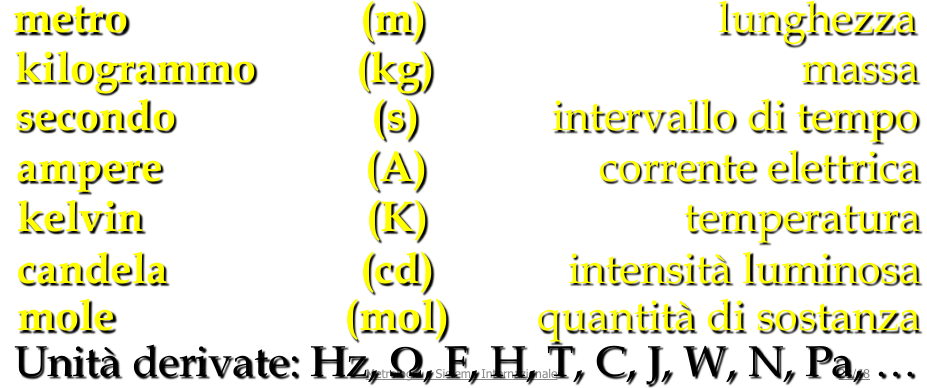
\includegraphics[
        width=12cm,
        height=6cm,
        keepaspectratio,
    ]{unitafondamentali.png}
    \caption{Le unità fondamentali del Sistema Internazionale.}
  \end{center}
\end{figure}
Il Sistema Internazionale è un \bf Sistema Coerente \rm in quanto tutte le sue unità derivate (qualunque grandezza G) si ricavano come prodotti e rapporti delle 7 unità di base, senza introdurre fattori moltiplicativi (come  $\pi,e,5\dots$).\\
Possiamo scrivere quindi che, indicando con "$dim(G)$" l'unità derivata dalle unità base SI: $$ dim(G) = L^\alpha M^\beta T^\gamma I^\delta \theta ^\varepsilon J^\eta N^\zeta  $$

Avendo:
\begin{itemize}
  \item L : Lunghezza (metro)
  \item M : Massa (kilogrammo)
  \item T : Intervallo di Tempo (secondo)
  \item I : Intensità di Corrrente (Ampere)
  \item $\theta$ : Temperatura (Kelvin)
  \item J : Intensità Luminosa (candela)
  \item N : Quantità di Sostanza (mole)
\end{itemize}

ognuno con il proprio esponente. Naturalmente, se la specifica unità base non compare nelle unità che compongono quella derivata, avrà esponente pari a $0$.
\\


Il Sistema Internazionale è anche un sistema completo? Tutte le unità di misura esistenti possono essere espresse attraverso le unità di base? Se così non fosse, sarebbe necessario aggiungere qualche unità a quelle del sistema internazionale.\\

Un'altra caratteristica importante del Sistema Internazionale è che le unità di base sono tra di loro dimensionalmente indipendenti, ma non logicamente indipendenti (e.g. il metro "dipende dal secondo").\\

Inoltre, nel S.I. esiste una sola unità di misura per ciascuna grandezza fisica, che è la corretta unità di misura di base o derivata da quelle di base. Ed è anche importante menzionare che attraverso uno qualsiasi dei \bf prefissi decimali approvati\rm, detti prefissi SI, può essere usato per costruire multipli e sottomultipli decimali delle unità di misura SI. Anche se sembra una caratteristica abbastanza naturale, esistono dei sistemi di misura che non la rispettano, ad esempio il sistema imperiale di misurazione delle distanze: la \it yard \rm non corrisponde a $1\ K\ inches$.

\subsubsection{Definzioni Assolute e Definizioni con Campioni Manufatti}
Nel Sistema Internazionale (ad oggi: settembre 2018), esistono ancora unità base definite attraverso dei campioni di riferimento, ad esempio il kilogrammo. Ebbene queste definzioni sono in un certo qual modo peggiori rispetto a quelle deifinite in modo assoluto, perché compromettendo il campione (ammettendo che esso sia unico, cosa che per fortuna non è - ne esistono diversi altri molto simili), si modificano virtualmente tutte le misure fatte da quel momento in poi. Un classico esempio espresso informalmente potrebbe essere "se qualcuno stanotte scambia il campione del kilogrammo, domani potremmo pesare tutti due etti in meno".

Le definizioni assolute invece sono "un'altra storia", perché esse sono realizzate attraverso costanti universali e proprietà invarianti della natura: il metro è definito attraverso la velocità della luce (costante universale), il secondo è definito attraverso la radiazione emessa da un atomo di Cesio in una particolare situazione (costante). Queste costanti (proprio per la loro natura di costanti) non varieranno mai nel tempo e si possono sempre ricavare.

\subsubsection{Cenni sulle Definizioni}
Prendendo come esempio la definzione dell'\bf Ampere\rm, la quale si basa sulla ricostruzione di un esperimento, abbiamo che la sua miglior realizzazione ha un'accuratezza di $10^{-7}$. Quest'accuratezza, confrontata con quella del secondo ($10^{-15}$) e del metro ($10^{-12}$ nella sua migliore realizzazione) risulta essere abbastanza scarsa. Questo è un gran contro della definizione dell'Ampere com'è adesso, perché tutte le unità di misura di tipo elettrico/elettronico si basano su di essa e quindi non si potrà mai avere una misura elettrica con un'accuratezza maggiore di $10^{-7}$.

In realtà, grazie agli effetti Josephson e Hall, si riescono a realizzare Volt Ohm con una riproducibilità altissima. Mentre la riproducibilità dell'Ampere è piuttosto scarsa, considerando che si dovrebbero porre in una stanza in cui si è simulato il vuoto due fili elettrici disposti in verticale di una lunghezza di almeno 10 metri.

\subsection{Tipi di Campioni}
Di seguito un elenco dei tipi di campioni che possiamo attualmente trovare in circolazione:s
\begin{itemize}
  \item \bf Campioni Primari: \rm sono quelli a cui si riferisce il Sistema Internazionale, che realizzano l'unità con i migliori livelli di accuratezza praticamente ottenibili.
  \item \bf Campioni Secondari: \rm consentono di trasferire l'unità ed effettuare i confronti tra i campioni primari e verso altri campioni. Se dobbiamo tarare uno strumento a Politecnico di Milano utiliziamo un campione secondario riferendoci a qualche ente nazionale.
  \item \bf Campioni di Trasferimento: \rm sono spesso campioni secondari, ma che sono anche adatti al trasporto.
  \item \bf Campioni "locali": \rm all'interno di un istituto a azienta, si dividono in campioni di prima linea (o di riferimento) e campioni di seconda linea (o di lavoro).
  \item \bf Campioni di Prima Linea: \rm si usano nei centri di taratura e di certificazione; sono usati oco di frequente e per tarare i campioni di seconda linea, oppure costutuiscono il campione di riferimento per l'istutito/azienda/laboratorio.
  \item \bf Campioni de Seconda Linea: \rm si usano nelle misure e confronti di routine, previo un confronto con quelli di prima linea, per fare le misure correnti (e.g. nella produzione o per misure sul campo).
\end{itemize}
Possiamo vedere questo elenco anche come una \it catena di riferibilità\rm, che abbiamo menzionato nella sezione precedente.

\subsection*{Taratura e Messa in Punto}
\begin{itemize}
  \item \bf Taratura: \rm consente di valutare l'incertezza di un campione/strumento rispetto a uno di qualità superiore e ricavare le correzioni (vedi Riferibilità).
  \item \bf Messa in Punto: \rm insieme di operazioni volte a permettere a uno strumento di operare nelle migliori condizioni di lavoro.
\end{itemize}
\section{Simboli e Regole del S.I.}
\begin{figure}[H]
  \begin{center}
    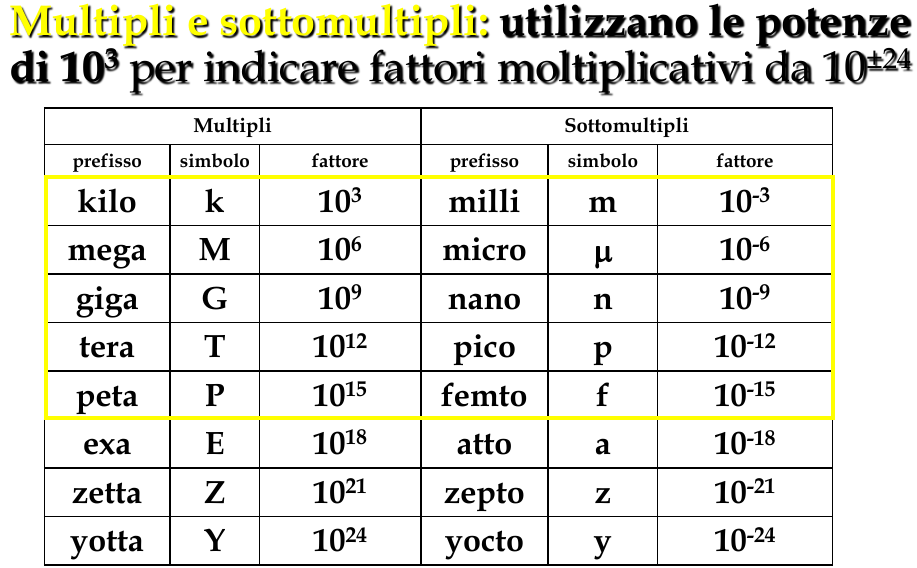
\includegraphics[
        width=12cm,
        height=6cm,
        keepaspectratio,
    ]{multiplisottomultipli.png}
    \caption{Multipli e Sottomultipli nel Sistema Internazionale.}
  \end{center}
\end{figure}
\subsection{Unità Logaritmiche}
Le unità logaritmiche esprimono sotto form di logaritmo il rapporto tra due grandezze \bf omogenee\rm. Notiamo che le grandezze in rapporto devono necessariamente essere omogenee, perché l'operatore logaritmo agisce solamente su numeri puri.
Una caratteristica che torna utile nelle unità logaritmiche è una delle proprietà dei logaritmi, cioè che le operazioni di moltiplicazione e divisione tra numeri si traducono in somme e differenze.

Le unità logaritmiche sono utilizzate molto el campo dell'elettrinica e delle telecomunicazioni. I logaritmi più comunemente utilizzati sono quello in base 10 ($log_{10}$), quello in base $e$ ($log_{e} = ln$) e in informatica quello in base 2 ($log_{2}$).
\subsubsection{Il Bel}
Il \textbf{bel} esprime il rapporto di potenze in scala logaritmica utilizzando una base decimale: $$\Bigg(\frac{P_{2}}{P_{1}}\Bigg)_{(bel)} = log_{10}\Bigg(\frac{P_{2}}{P_{1}}\Bigg)$$
Il nome "bel" deriva dal suo inventore \textit{Alexander Graham-Bell} il quale, dovendo fare dei confronti tra potenze trasmesse per via aerea, si accorse che decadevno in maniera esponenziale.\\
È molto importante ricordarsi sempre che il bel rappresenta il logaritmo di un \textbf{rapporto tra due misure}, ed è quindi un modo per mettere in relazione due misure. Il difetto principale del bel è che 1 bel rappresenta un rapporto di un fattore 10:1 e dunque una scala in bel risulta "grossolana". Per risolvere \footnotetext[1]{Il significato di "risolvere" in questo caso è legato alla definizione che abbiamo dato nella sezione 1.3. Quindi "risolvere" in questo contesto và interpretato come "avere una \textbf{risoluzione} tale da poter apprezzare variazioni "più fini".} rapporti o variazioni "più fini" è conveniente utilizzare un suo \textbf{sottomultiplo}, il \textit{deciBel (dB)}.
\subsubsection{Il deciBel}
È un \textit{sottomultiplo} ($\frac{1}{10}$) del bel, esprime quindi anch'esso il rapporto di potenze (o anche ampiezze), mediante il logaritmo in base 10. $$\Bigg(\frac{P_{2}}{P_{1}}\Bigg)_{(dB)} = 10log_{10}\Bigg(\frac{P_{2}}{P_{1}}\Bigg)$$
Ricordando che il deciBel, come il bel, esprime rapporti di potenze, possiamo dire che $ 1\ dB \simeq 1.25 = 1 + 25\% $. Quindi si può dire che $P_{2}$ è "più grande" di $P_{1}$ del 25\%.\\
I rapporti di ampiezze, quando tensione e correnti sono misurate \textbf{su uno stesso carico}, si esprimo in deciBel secondo la relazione $$ 20log_{10}\Bigg(\frac{A_{2}}{A_{1}}\Bigg) $$
Questa fotumla discende direttamente dal decibel.$$Inserire\  dimostrazione?????$$
\subsubsection*{"dBx"}
Con dBx si indica il valore in decibel epsresso rispetto ad un \textbf{riferimento x}. Scelto un livello di potenza $P_{x}$ come riferimento, un qualunque valore di potenza P può essere espresso in \textbf{decibel rispetto al riferimento} come $$ P_{(dBx} = 10log_{10}\Bigg( \frac{P}{P_{x}} \Bigg) $$
In particolare, esisterano dunque:
$$P_{(dBm)} = 10log_{10}\Bigg( \frac{P}{1mW} \Bigg)$$
$$P_{(dBW)} = 10log_{10}\Bigg( \frac{P}{1W} \Bigg)$$
$$P_{(dBk)} = 10log_{10}\Bigg( \frac{P}{1kW} \Bigg)$$
Che esprimono la variazione della potenza misurata rispetto ad un riferimento "standard" di 1 milliWatt, Watt oppure kiloWatt.
\subsubsection*{Calcoli Approssimati con i dB ????}
\end{document}
